%\documentclass[aps,prb,twocolumn,superscriptaddress,preprintnumbers,amsmath,amssymb,floatfix]{revtex4}
\documentclass[aps,prb,preprint,superscriptaddress,amsmath,amssymb,floatfix]{revtex4}
%\documentclass[aps,prl,onecolumn,groupedaddress,amsmath,amssymb,12pt]{revtex4}
\usepackage{graphicx}
\usepackage{ifthen}
\usepackage{dcolumn}% Align table columns on decimal point
\usepackage{bm}% bold math
\usepackage{multirow}
\usepackage{booktabs}
\usepackage{bm}% bold math
\usepackage{amsbsy}
\usepackage{amsmath}
\usepackage{amssymb}
\usepackage{subfigure}


%Definition of new commands
\newcommand{\f}[2]{\ensuremath{\frac{\displaystyle{#1}}{\displaystyle{#2}}}}
\newcommand{\lr}[1]{\langle{#1}\rangle}
\newcommand{\colv}[2] {\left(\begin{array}{c} #1 \\ #2 \end{array}\right)}
\renewcommand{\thefootnote}{\fnsymbol{footnote}}
\newcommand{\be} {\begin{eqnarray}}
\newcommand{\ee} {\end{eqnarray}}
%--------------------------------------------------------------------------
%EQ COMMANDS
%--------------------------------------------------------------------------
\newcommand{\two}{\mspace{-2.0mu}}
\newcommand{\four}{\mspace{-4.0mu}}
\newcommand{\plus}{\mspace{-4.5mu}+\mspace{-3.5mu}}
\newcommand{\minus}{\mspace{-4.5mu}-\mspace{-3.5mu}}
\newcommand{\pp}{'\mspace{-2.0mu}'}
\newcommand{\xlb}[4]{#1\ifthenelse{\equal{#2}{0}}{}{_{\alpha #2}}
\mspace{-2.0mu}\genfrac{(}{)}{0pt}{1}{\ifthenelse{\equal{#3}{0}}{0}{l #3}} 
{\ifthenelse{\equal{#4}{0}}{0}{b #4}}}

\newcommand{\xkv}[4]{#1\mspace{-5.0mu}\left(\mspace{-8.0mu}
\begin{smallmatrix}#2\four{}\four{}\mspace{-8.0mu}&\pmb{\kappa}#3\\&\nu 
#4\end{smallmatrix}\mspace{-5.0mu}\right)}

\newcommand{\evect}[6]{#1\mspace{-4.0mu}\left(\mspace{-8.0mu}
\begin{smallmatrix}#2\mspace{-8.0mu}&\pmb{\kappa} #3 &b #5\\&\nu #4 &
\alpha #6\end{smallmatrix}\mspace{-5.0mu}\right)}

\newcommand{\varmat}[8]{\mspace{-5.0mu}\left(\mspace{-8.0mu}
\begin{smallmatrix}\ifthenelse{\equal{#3}{0}}{\mspace{-8.0mu}&b_{#1}&b_{#2}
\\&\alpha_{#1}&\alpha_{#2}} {\ifthenelse{\equal{#7}{0}}{#1\mspace{-8.0mu}&
\pmb{\kappa}#2#3\mspace{-8.0mu}&\pmb{\kappa}#4#5\mspace{-8.0mu}&\pmb{\kappa}
#6\\&\nu#2&\nu#4&\nu#6} {#1\mspace{-8.0mu}&\pmb{\kappa}#2#3\mspace{-8.0mu}&
\pmb{\kappa}#4#5\mspace{-8.0mu}&\pmb{\kappa}#6#7\mspace{-8.0mu}&\pmb{\kappa}
#8\\&\nu#2&\nu#4&\nu#6&\nu#8}}\end{smallmatrix}\mspace{-5.0mu}\right)}

\newcommand{\EXP}[1]{\exp\mspace{-5.0mu}\left[#1\right]\mspace{-3.0mu}}

\newcommand{\tpp}[2]{\left(\mspace{-2.0mu}\xkv{\omega}{}{}{}#1\xkv{\omega}
{}{'}{'}#2\xkv{\omega}{}{\pp}{\pp}\mspace{-2.0mu}\right)}



%--------------------------------------------------------------------------
\newcommand{\SUM}[2]{\ifthenelse{\equal{#1}{0}}{\sum_{
\alpha_{#2},b_{#2},l_{#2}}^{3,n,N}} {\ifthenelse{\equal{#1}{1}}{\sum_{
\alpha_{#2},b_{#2}}^{3,n}}{\sum_{\pmb{\kappa}#2,\nu#2}^{N,3n}}}}

\newcommand{\SUMprime}[2]{\ifthenelse{\equal{#1}{0}}
{\sum_{\alpha_{#2},b_{#2},l_{#2}}^{3,n,N}} 
{\ifthenelse{\equal{#1}{1}}{\sum_{\alpha_{#2},b_{#2}}^{3,n}}
{\sum_{\pmb{\kappa}^{'}#2,\nu#2}^{N,3n}}}}

\newcommand{\SUMalpha}[2]{\ifthenelse{\equal{#1}{0}}
{\sum_{\alpha_{#2}}^{3}} {\ifthenelse{\equal{#1}{1}}
{\sum_{\alpha_{#2},b_{#2}}^{3,n}}{\sum_{\pmb{\kappa}#2,\nu#2}^{N,3n}}}}
%--------------------------------------------------------------------------
\newcommand{\SUMalphap}[2]{\ifthenelse{\equal{#1}{0}}
{\sum_{\alpha'_{#2}}^{3}} {\ifthenelse{\equal{#1}{1}}
{\sum_{\alpha'_{#2},b'_{#2}}^{3,n}}{\sum_{\pmb{\kappa}#2,\nu#2}^{N,3n}}}}

\newcommand{\SUMb}[2]{\ifthenelse{\equal{#1}{0}}{\sum_{b_{#2}}^{n}}
 {\ifthenelse{\equal{#1}{1}}{\sum_{\alpha_{#2},b_{#2}}^{3,n}}
{\sum_{\pmb{\kappa}#2,\nu#2}^{N,3n}}}}

\newcommand{\SUMbp}[2]{\ifthenelse{\equal{#1}{0}}{\sum_{b'_{#2}}^{n}}
 {\ifthenelse{\equal{#1}{1}}{\sum_{\alpha'_{#2},b'_{#2}}^{3,n}}
{\sum_{\pmb{\kappa}#2,\nu#2}^{N,3n}}}}

\newcommand{\SUMl}[2]{\ifthenelse{\equal{#1}{0}}{\sum_{l_{#2}}^{N}}
 {\ifthenelse{\equal{#1}{1}}{\sum_{\alpha_{#2},b_{#2}}^{3,n}}
{\sum_{\pmb{\kappa}#2,\nu#2}^{N,3n}}}}

\newcommand{\SUMlp}[2]{\ifthenelse{\equal{#1}{0}}{\sum_{l'_{#2}}^{N}}
 {\ifthenelse{\equal{#1}{1}}{\sum_{\alpha'_{#2},b'_{#2}}^{3,n}}
{\sum_{\pmb{\kappa}#2,\nu#2}^{N,3n}}}}

\newcommand{\abcdt}[5]{\mspace{-4.0mu}\left(\mspace{-8.0mu}
\begin{smallmatrix}&\ifthenelse{\equal{#1}{}}{a}{#1}&\ifthenelse
{\equal{#3}{}}{c}{#3}\\&\ifthenelse{\equal{#2}{}}{b}{#2}&\ifthenelse
{\equal{#4}{}}{d}{#4}\end{smallmatrix}\mspace{-2.0mu};\ifthenelse
{\equal{#5}{}}{t}{#5}\right)}

\newcommand{\abcd}[4]{\mspace{-4.0mu}\left(\mspace{-8.0mu}
\begin{smallmatrix}&\ifthenelse{\equal{#1}{}}{a}{#1}&\ifthenelse
{\equal{#3}{}}{c}{#3}\\&\ifthenelse{\equal{#2}{}}{b}{#2}&\ifthenelse
{\equal{#4}{}}{d}{#4}\end{smallmatrix}\mspace{-3.0mu}\right)}

\newcommand{\abt}[3]{\mspace{-4.0mu}\left(\mspace{-8.0mu}\begin
{smallmatrix}&\ifthenelse{\equal{#1}{}}{a}{#1} \\&\ifthenelse{
\equal{#2}{}}{b}{#2}\end{smallmatrix}\mspace{-2.0mu};
\ifthenelse{\equal{#3}{}}{t}{#3}\right)}

\newcommand{\ab}[2]{\mspace{-4.0mu}\left(\mspace{-8.0mu}
\begin{smallmatrix}&\ifthenelse{\equal{#1}{}}{a}{#1} \\&\ifthenelse
{\equal{#2}{}}{b}{#2}\end{smallmatrix}\mspace{-3.0mu}\right)}

\newcommand{\kvbat}{\mspace{-4.0mu}\left(\mspace{-8.0mu}
\begin{smallmatrix} &\pmb{\kappa} &b \\ &\nu &\alpha\end{smallmatrix}
\mspace{-2.0mu};t\right)}
%--------------------------------------------------------------------------
\newcommand{\kvbatp}{\mspace{-4.0mu}\left(\mspace{-8.0mu}
\begin{smallmatrix} &\pmb{\kappa} &b' \\ &\nu &\alpha'\end{smallmatrix}
\mspace{-2.0mu};t\right)}

\newcommand{\kvbaw}{\mspace{-4.0mu}\left(\mspace{-8.0mu}
\begin{smallmatrix} &\pmb{\kappa} &b \\ &\nu &\alpha\end{smallmatrix}
\mspace{-2.0mu};\omega\right)}

\newcommand{\kvbawp}{\mspace{-4.0mu}\left(\mspace{-8.0mu}
\begin{smallmatrix} &\pmb{\kappa} &b' \\ &\nu &\alpha'\end{smallmatrix}
\mspace{-2.0mu};\omega\right)}

\newcommand{\kvba}{\mspace{-4.0mu}\left(\mspace{-8.0mu}
\begin{smallmatrix} &\pmb{\kappa} &b \\ &\nu &\alpha\end{smallmatrix}
\mspace{-3.0mu}\right)}

\newcommand{\kvbap}{\mspace{-4.0mu}\left(\mspace{-8.0mu}
\begin{smallmatrix} &\pmb{\kappa} &b' \\ &\nu &\alpha'\end{smallmatrix}
\mspace{-3.0mu}\right)}
%--------------------------------------------------------------------------
\newcommand{\kpvba}{\mspace{-4.0mu}\left(\mspace{-8.0mu}
\begin{smallmatrix} &\pmb{\kappa}^{'} &b \\ &\nu &\alpha\end{smallmatrix}
\mspace{-3.0mu}\right)}

\newcommand{\kva}{\mspace{-4.0mu}\left(\mspace{-8.0mu}
\begin{smallmatrix} &\pmb{\kappa} \\ &\nu &\alpha\end{smallmatrix}
\mspace{-3.0mu}\right)}

\newcommand{\kvap}{\mspace{-4.0mu}\left(\mspace{-8.0mu}
\begin{smallmatrix} &\pmb{\kappa} \\ &\nu &\alpha'\end{smallmatrix}
\mspace{-3.0mu}\right)}

\newcommand{\kvb}{\mspace{-4.0mu}\left(\mspace{-8.0mu}
\begin{smallmatrix} &\pmb{\kappa} &b \\ &\nu \end{smallmatrix}
\mspace{-3.0mu}\right)}

\newcommand{\kvbp}{\mspace{-4.0mu}\left(\mspace{-8.0mu}
\begin{smallmatrix} &\pmb{\kappa} &b' \\ &\nu \end{smallmatrix}
\mspace{-3.0mu}\right)}

\newcommand{\kvt}{\mspace{-4.0mu}\left(\mspace{-8.0mu}
\begin{smallmatrix}&\pmb{\kappa} \\&\nu\end{smallmatrix}
\mspace{-2.0mu};t\right)}

\newcommand{\kpvt}{\mspace{-4.0mu}\left(\mspace{-8.0mu}
\begin{smallmatrix}&\pmb{\kappa}^{'} \\&\nu\end{smallmatrix}
\mspace{-2.0mu};t\right)}

\newcommand{\kvw}{\mspace{-4.0mu}\left(\mspace{-8.0mu}
\begin{smallmatrix}&\pmb{\kappa} \\&\nu\end{smallmatrix}
\mspace{-2.0mu};\omega\right)}

\newcommand{\kv}{\mspace{-4.0mu}\left(\mspace{-8.0mu}
\begin{smallmatrix}&\pmb{\kappa} \\&\nu\end{smallmatrix}
\mspace{-3.0mu}\right)}

\newcommand{\kw}{\mspace{-4.0mu}\left(\mspace{-8.0mu}
\begin{smallmatrix}&\pmb{\kappa} \\&\omega\end{smallmatrix}
\mspace{-3.0mu}\right)}

\newcommand{\kpvp}{\mspace{-4.0mu}\left(\mspace{-8.0mu}
\begin{smallmatrix}&\pmb{\kappa'} \\&\nu'\end{smallmatrix}
\mspace{-3.0mu}\right)}
%--------------------------------------------------------------------------
\newcommand{\lbt}{\mspace{-4.0mu}\left(\mspace{-8.0mu}
\begin{smallmatrix}&l \\&b\end{smallmatrix}\mspace{-2.0mu};t\right)}

\newcommand{\lbtp}{\mspace{-4.0mu}\left(\mspace{-8.0mu}
\begin{smallmatrix}&l' \\&b'\end{smallmatrix}\mspace{-2.0mu};t\right)}

\newcommand{\lt}{\mspace{-4.0mu}\left(\mspace{-8.0mu}
\begin{smallmatrix}&l\end{smallmatrix}\mspace{-2.0mu};t\right)}

\newcommand{\ltp}{\mspace{-4.0mu}\left(\mspace{-8.0mu}
\begin{smallmatrix}&l'\end{smallmatrix}\mspace{-2.0mu};t\right)}

\newcommand{\lb}{\mspace{-4.0mu}\left(\mspace{-8.0mu}
\begin{smallmatrix}&l \\&b\end{smallmatrix}\mspace{-3.0mu}\right)}

\newcommand{\lbp}{\mspace{-4.0mu}\left(\mspace{-8.0mu}
\begin{smallmatrix}&l' \\&b'\end{smallmatrix}\mspace{-3.0mu}\right)}
%--------------------------------------------------------------------------
%COMMANDS
%--------------------------------------------------------------------------

%--------------------------------------------------------------------------
\begin{document}
%--------------------------------------------------------------------------

%--------------------------------------------------------------------------
\title{Evaluation of the Virtual Crystal Approximation}
%--------------------------------------------------------------------------
\author{Jason M. Larkin}
\affiliation{Department of Mechanical Engineering\\Carnegie Mellon 
University\\Pittsburgh, PA 15213}
\author{A. J. H. McGaughey}
\email{mcgaughey@cmu.edu}
\affiliation{Department of Mechanical Engineering\\
Carnegie Mellon University\\Pittsburgh, PA 15213}
%--------------------------------------------------------------------------

%--------------------------------------------------------------------------
\date{\today}
%--------------------------------------------------------------------------


%--------------------------------------------------------------------------
\begin{abstract}
%--------------------------------------------------------------------------

%--------------------------------------------------------------------------
\end{abstract}
%--------------------------------------------------------------------------


%--------------------------------------------------------------------------
\maketitle
%--------------------------------------------------------------------------
\clearpage
%--------------------------------------------------------------------------
\section{\label{S:Intro}Introduction}
%--------------------------------------------------------------------------

For thermolectric device applications, minimizing a thermoelectric 
material's thermal 
conductivity has become a promising technique for increasing $ZT>3$.
\cite{chen_recent_2003,dresselhaus_new_2007} In semiconductor alloys, 
understanding the effect of disorder is necessary for optimizing 
ZT by further lowering thermal conductivity.
\cite{he_thermoelectric_2006,huang_filler-reduced_2010,
toberer_phonon_2011,tian_phonon_2012}

Recently, work using ab-initio calculations\cite{garg_role_2011}

Abeles introduced the idea of using a virtual crystal to replace 
a disordered one, computing the
thermal conductivity of Si/Ge alloys by treating both
disorder and anharmonicity as perturbations.
\cite{abeles_lattice_1963} 

The goal of this work is to verify the 


%--------------------------------------------------------------------------
\section{\label{S:Lifetimes}Kinetic Theory}
%--------------------------------------------------------------------------

For a perfect system, all vibrational modes are phonons.

Diffusons, locons and propagons \cite{allen_diffusons_1999}.

\begin{equation}\label{EQ:M:k_mode}
\begin{split}
k_{vib,\mathbf{n}}=&\sum_{\pmb{\kappa}} \sum_\nu c_{ph}\kv 
\pmb{v}^{2}_{g,\mathbf{n}}\kv \tau\kv.
\end{split}
\end{equation}

Here, $c_{ph}$ is the phonon volumetric specific heat and 
${v}_{g,\mathbf{n}}$ is
the component of the group velocity vector in direction $\mathbf{n}$. 
Since the systems we consider are classical and obey Maxwell-Boltzmann 
statistics,\cite{mcquarrie2000} the
specific heat is $k_{B}/V$ per mode in the harmonic limit where $V$ 
is the system volume. This approximation is used here and has been shown 
to be suitable for LJ argon\cite{mcgaughey2004c} and SW silicon.
\cite{goicochea2010}

Finally, we adopt the single-mode relaxation
time approximation [16] as an approximate solution of
the Boltzmann transport equation [17,18];

Abeles introduced the idea of using a virtual (perfect) crystal 
to replace a disordered one, computing the
thermal conductivity of Si/Ge alloys by treating both
disorder and anharmonicity as perturbations.
\cite{abeles_lattice_1963} 

%--------------------------------------------------------------------------
\subsection{\label{S:}Phonon Group Velocities}
%--------------------------------------------------------------------------
The group velocity vector is the gradient of the dispersion curves 
(i.e., $\partial \omega / \partial \pmb{\kappa}$), which can be 
calculated from the frequencies and wavevectors using finite differences. 
In this work, the group velocities are calculated using finite difference 
and quasi-harmonic lattice dynamics because a very small finite difference 
can be used which reduces the error.\cite{mcgaughey2006b} 

Of particular interest if the phonon mean free path (MFP),

\begin{equation}\label{EQ:M:phonon_mfp}
\begin{split}
\Lambda\kv = |\pmb{v}_{g}| \tau\kv,
\end{split}
\end{equation}

which requires a group velocity.
%--------------------------------------------------------------------------
\subsection{\label{S:}Phonon Lifetimes}
%--------------------------------------------------------------------------

\begin{equation}\label{EQ:M:tau_matthiessen}
\frac{1}{\tau} = \frac{1}{\tau_{p-p}} + \frac{1}{\tau_{b}} + 
\frac{1}{\tau_{d}},
\end{equation}
where $\tau_{p-p}$ accounts for phonon-phonon scattering, $\tau_{b}$ 
accounts for boundary scattering, $\tau_{d}$ accounts for defect 
scattering.

\begin{equation}\label{EQ:M:tau_b}
\tau_{b} = L/v_g.
\end{equation}

Phonon-phonon scattering ($\tau_{p-p}$) is typically treated 
using anharmonic perturbation theory including only 3-phonon 
processes.\cite{turney_predicting_2009,garg_role_2011,tian_phonon_2012} 
At low frequencies,
$\tau_{p-p}$ follows a scaling due to both normal ($B_1\omega^2$) 
and umklapp ($B_2\omega^2$) 3-phonon scattering processes, where 
the density of states is Debye-like. The 
constants $B_1$ and $B_2$ are typically fit to experimental data.
 Higher 
order n-phonon process can become important at higher temperatures.
\cite{turney_predicting_2009} 

At low frequencies, the phonon scattering due to point-defects is 
given by
\begin{equation}\label{EQ:M:tau_d_D}
\frac{1}{\tau_{d}} = \frac{V \omega^4}{4 \pi v_p^2 v_g} 
( \sum_i c_i(1-m_i/\bar m)^2 + \sum_i c_i(1-r_i/\bar r)^2 ),
\end{equation}

\begin{equation}\label{EQ:M:tau_d_D}
\frac{1}{\tau_{d}} = \frac{V \omega^4}{4 \pi v_p^2 v_g} 
\sum_i c_i(1-m_i/\bar m)^2 ,
\end{equation}

where $c_i$ is the fraction, $m_i$ is the mass, and $r_i$ is the radius 
(scattering cross-section) 
of species i and $\bar r$ is the average atomic radius.
\cite{klemens_scattering_1955,klemens_thermal_1957} 
The frequency dependence is the same as 
Rayleigh scattering, which is valid at low frequency in the Debye limit.

For all frequencies, Tamura gives a general expression for 
point defect scattering which is harmonic \cite{tamura_isotope_1983}

\begin{equation}\label{EQ:M:tau_d}
\frac{1}{\tau_{d}\kv} = \frac{\pi}{2N}\omega_{\mathbf{q}s}^2 
\sum_{\mathbf{q'}s'} \delta( \omega_{\mathbf{q}s} - 
\omega_{\mathbf{q'}s'} ) \sum_{b} g(b) 
|e_{\mathbf{q'}s'}^*(b) \cdot e_{\mathbf{q}s}(b) |^2 ,
\end{equation}

where 
$g(b) = \sum_i c_i(b)(1-m_i(b)/\bar m(b))^2$

N is the number of unit cells.

Though the
expression for harmonic scattering [Eq. (2)] is valid for
small mass disorder, its use leads to good agreement with
experimentally measured phonon linewidths, even in the
case of the Ni0:55 Pd0:45 alloy, where the atomic species
are chemically similar but mass disorder is large
(mPd =mNi 1⁄4 1:812) [20].

Cahill shows that even though the mass difference between Si and Ge is 
larger than the mass of Si, the defect scaling agrees with experimental 
measurements of thermal conductivity in dilute SiGe epitaxial layers.
\cite{cahill_thermal_2005}
%--------------------------------------------------------------------------
\section{\label{S:}Virtual Crystal Approximation}
%--------------------------------------------------------------------------
We calculate at all compositions
the phonon modes of the virtual crystal (which has
a lattice parameter, mass, and
force constants of that particular composition)
and derive from those the frequencies, group velocities,
and lifetimes to calculate thermal
conductivity.

Garg show that the virtual crystal approximation works well for Si-Ge 
\cite{garg_role_2011}

%--------------------------------------------------------------------------
\subsection{\label{S:}Mass vs Bond Disorder}
%--------------------------------------------------------------------------
The decreased vibrational conductivity of systems which are highly 
anharmonic, such as weak covalently and Van der Waals bonded systems,
\cite{} is 
accounted for by the Gruneisen parameter. For a purely harmonic system, 
the mode specific Gruneisen parameter is zero and the phonon lifetimes 
are infinite.

Cahill shows that conductivty of Ge-doped Si epitaxial layers agrees with 
the defect scaling cross section is captured mostly by the mass disorder.
\cite{cahill_thermal_2004}

The effect of bond and mass disorder has been investigated by Skye and 
Schelling for  
Si/Ge \cite{skye_thermal_2008}, where it was shown that mass disorder is 
the dominant scattering mechanism. Also, a first principle study of Si/Ge
demonstrates that virtual crystal approxmation Marzari 
Si/Ge PRL \cite{garg_role_2011}.  
A detailed study of PbTe/PbSe systems demonstrate the importance 
of bond environment for alloys.\cite{garg_phonon_2012}
%--------------------------------------------------------------------------
\subsection{\label{S:}VC and Gamma DOS Comparison}
%--------------------------------------------------------------------------
Bouchard show that alloy DOS varies smoothly with concentration.
\cite{bouchard_vibrational_1988}
%--------------------------------------------------------------------------
\subsection{\label{S:}Structure Factor of Gamma Point Modes}
%--------------------------------------------------------------------------
Demonstrates the importance of dispersion, even along different lattice 
directions ([100 vs [111]).

\begin{equation}\label{EQ:M:EL}
E^L\kv = 
\left|
\sum_{l,b} 
\hat{\mathbf{\kappa}} \cdot e\kvba 
\EXP{i\pmb{\kappa}\cdot\mathbf{r}_0\ab{l}{b}} 
\right|^2
\end{equation}

\begin{equation}\label{EQ:M:EL}
E^T\kv = 
\left|
\sum_{l,b} 
\hat{\mathbf{\kappa}} \times e\kvba 
\EXP{i\pmb{\kappa}\cdot\mathbf{r}_0\ab{l}{b}} 
\right|^2
\end{equation}

\begin{equation}\label{EQ:M:SL}
S^{L,T}\kw = 
\sum_{\nu} E^{L,T}\kv
\delta (\omega-\omega\kv)
\end{equation}

%--------------------------------------------------------------------------
\begin{figure}
\begin{center}
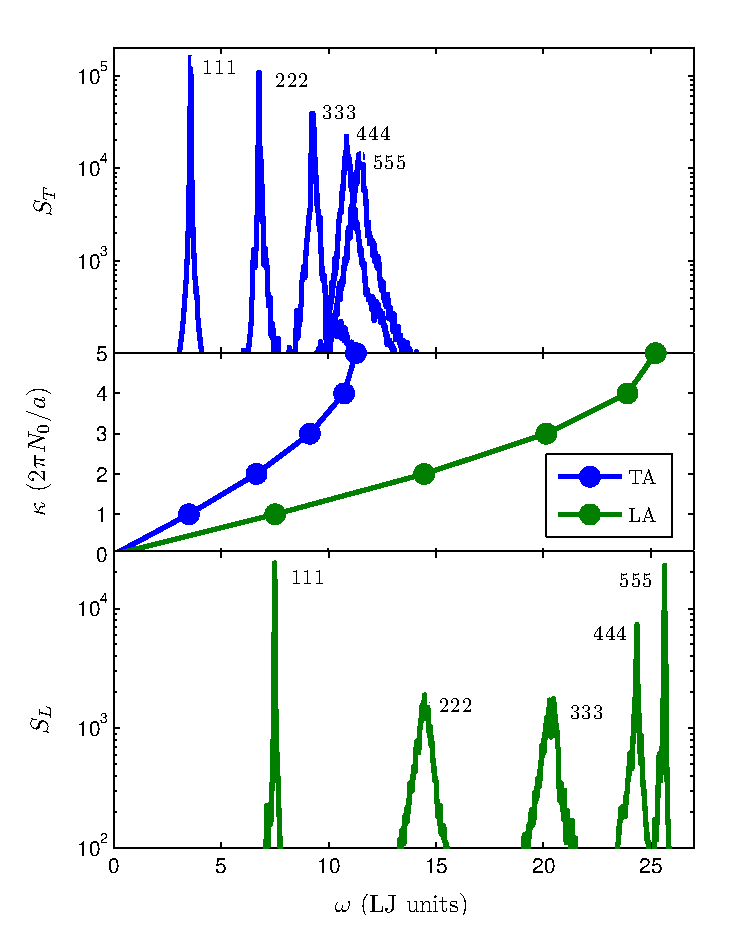
\includegraphics[scale=0.6]
{/home/jason/disorder/lj/alloy/m_dsf_plot_disp_c0.05_111.eps}
\vspace*{-5mm}
\end{center}
\caption{\label{FIG:phonon_diff} virtual crystal results}
\end{figure}
%--------------------------------------------------------------------------

%--------------------------------------------------------------------------
\begin{figure}
\begin{center}
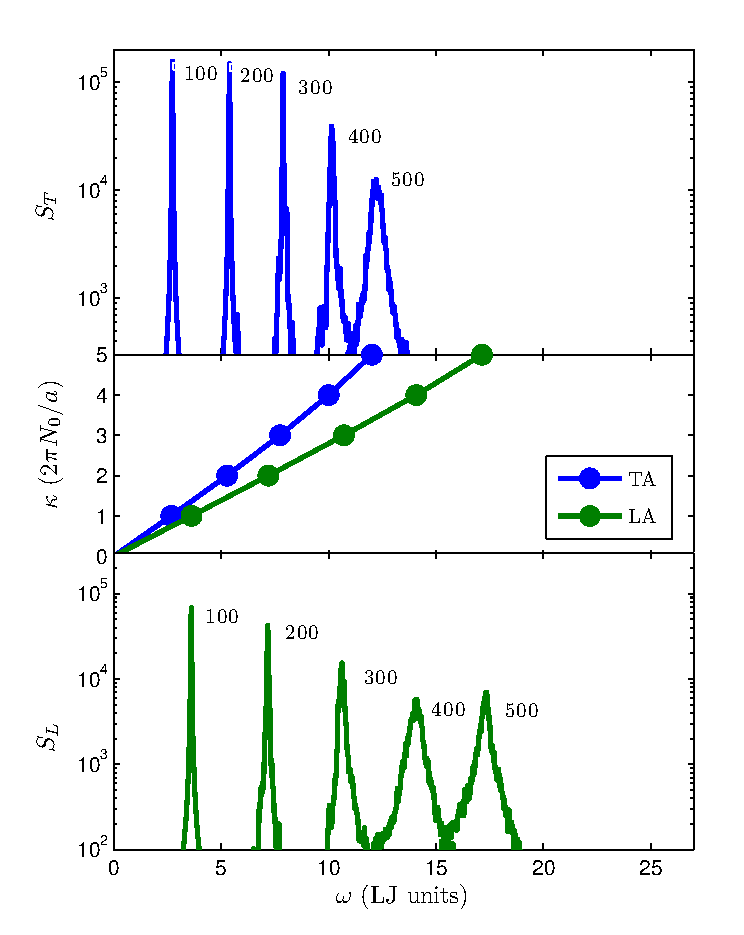
\includegraphics[scale=0.6]
{/home/jason/disorder/lj/alloy/m_dsf_plot_disp_c0.05_100.eps}
\vspace*{-5mm}
\end{center}
\caption{\label{FIG:phonon_diff} virtual crystal results}
\end{figure}
%--------------------------------------------------------------------------

%--------------------------------------------------------------------------
\begin{figure}
\begin{center}
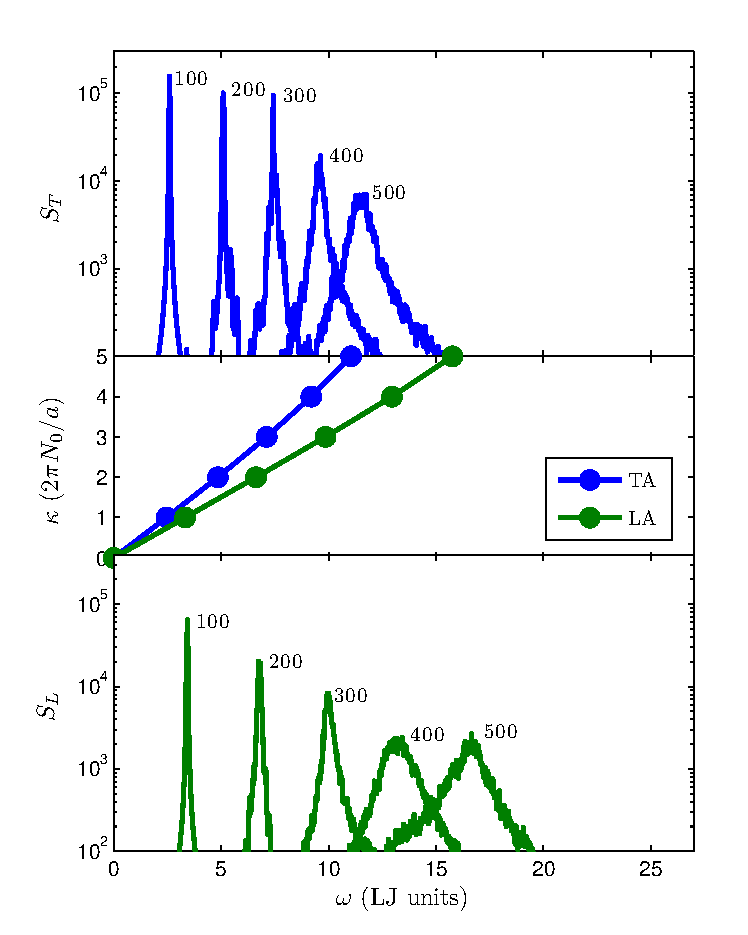
\includegraphics[scale=0.6]
{/home/jason/disorder/lj/alloy/m_dsf_plot_disp_c0.15_100.eps}
\vspace*{-5mm}
\end{center}
\caption{\label{FIG:phonon_diff} virtual crystal results}
\end{figure}
%--------------------------------------------------------------------------

%--------------------------------------------------------------------------
\begin{figure}
\begin{center}
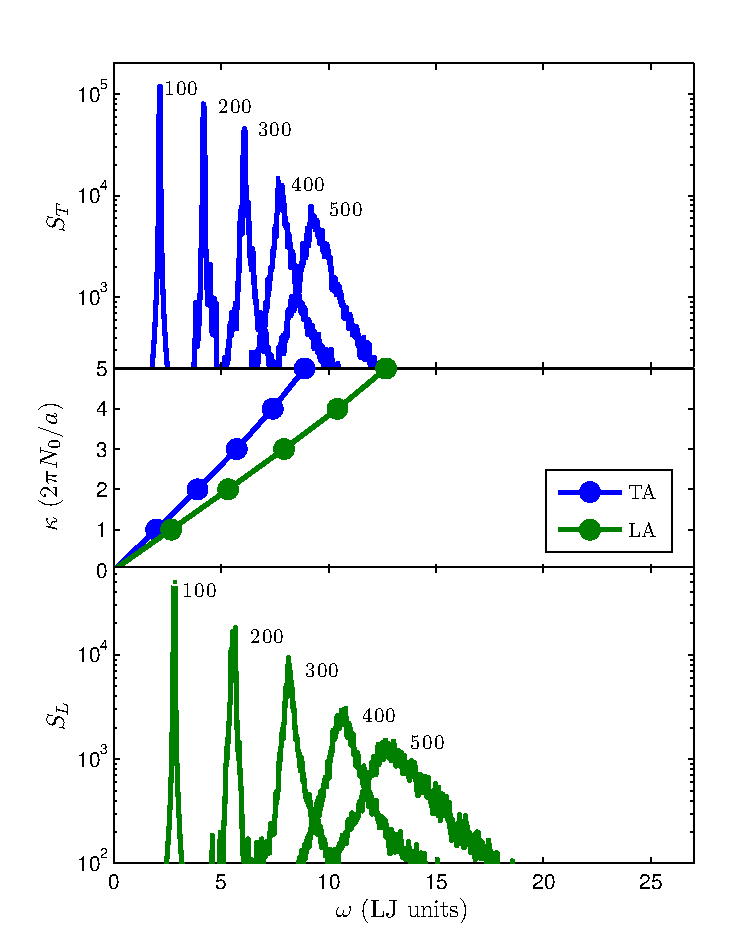
\includegraphics[scale=0.6]
{/home/jason/disorder/lj/alloy/m_dsf_plot_disp_c0.5_100.eps}
\vspace*{-5mm}
\end{center}
\caption{\label{FIG:phonon_diff} virtual crystal results}
\end{figure}
%--------------------------------------------------------------------------


%--------------------------------------------------------------------------
\subsection{\label{S:}Group Velocity}
%--------------------------------------------------------------------------
In ordered systems, the group velocity generally scales with both the 
density and stiffness of the material. For example, 
the reduced vibrational conductivity of Ge compared to Si can 
be (partially) explained in both in terms of the $\bar m$ 
(germanium has a larger density $\rho$ than silicon) 
and the group velocity (germanium has a smaller bulk modulus $B$, 
and $v_g \propto \sqrt{B/\rho}$.
Thus, for alloys, there should also be a corrsponding scaling 
of the group velocity with the alloy's concentration (mass
density).
Duda shows the reduction in group velocity of disordered systems.
\cite{duda_reducing_2011}
%--------------------------------------------------------------------------
\subsection{\label{S:Lifetimes}VC and Gamma Point Phonon Lifetimes}
%--------------------------------------------------------------------------

%--------------------------------------------------------------------------
\begin{figure}
\begin{center}
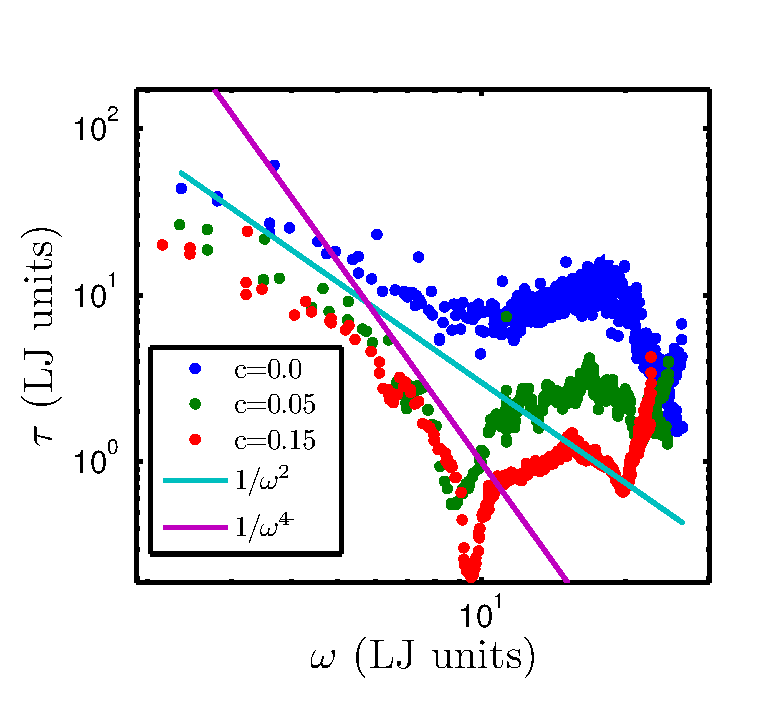
\includegraphics[scale=0.6]
{/home/jason/disorder/lj/alloy/xcorr_alloy_vc_life.eps}
\vspace*{-5mm}
\end{center}
\caption{\label{FIG:phonon_diff} virtual crystal results}
\end{figure}
%--------------------------------------------------------------------------

%--------------------------------------------------------------------------
\begin{figure}
\begin{center}
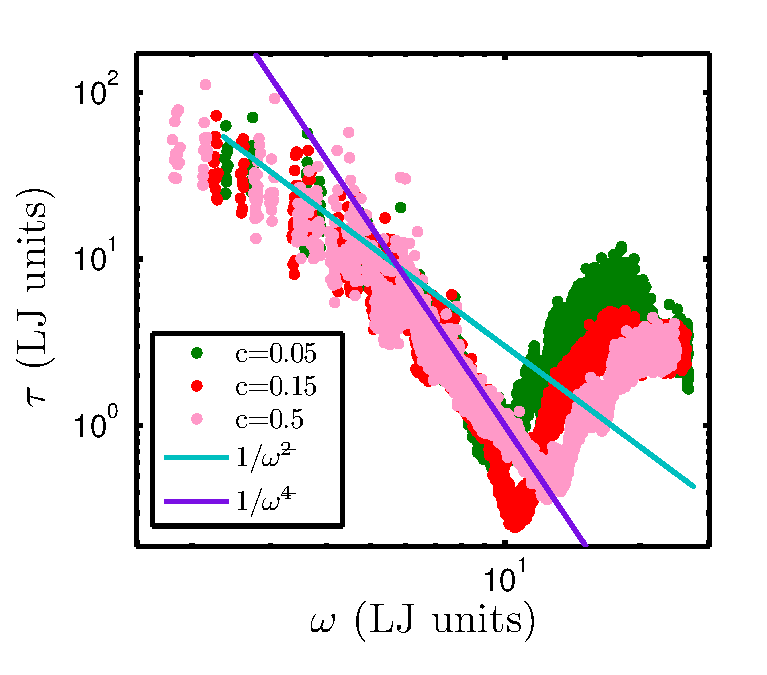
\includegraphics[scale=0.6]
{/home/jason/disorder/lj/alloy/xcorr_alloy_gamma_life.eps}
\vspace*{-5mm}
\end{center}
\caption{\label{FIG:phonon_diff} gamma point results}
\end{figure}
%--------------------------------------------------------------------------
\vspace{60mm}
%--------------------------------------------------------------------------
\section{\label{S:Lifetimes}Thermal Conductivity Predictions}
%--------------------------------------------------------------------------
The thermal conductivity of amorphous solids at low temperatures contain 
quantum statistical effects.\cite{freeman_thermal_1986} Molecular dynamics 
simulations are not able to capture quantum statistical effects.
%--------------------------------------------------------------------------
\subsection{\label{S:Lifetimes}From Molecular Dynamics}
%--------------------------------------------------------------------------
An addition of as little as 10\% Ge is sufficient to reduce the thermal 
conductivity to the minimum value achievable through alloying. 
Theoretically, mass disorder is found to increase the 
anharmonic scattering of phonons 
through a modification of their vibration eigenmodes. 
Notably, the thermal conductivity is found
to drop sharply after only a small amount of alloying. This
is due to the strong harmonic scattering of phonons even
in the dilute alloy limit.

Duda shows that taking a perfect alloy and disordering via an order 
parameter allows control of thermal conductivity.
\cite{duda_controlling_2012}
%--------------------------------------------------------------------------
\begin{figure}
\begin{center}
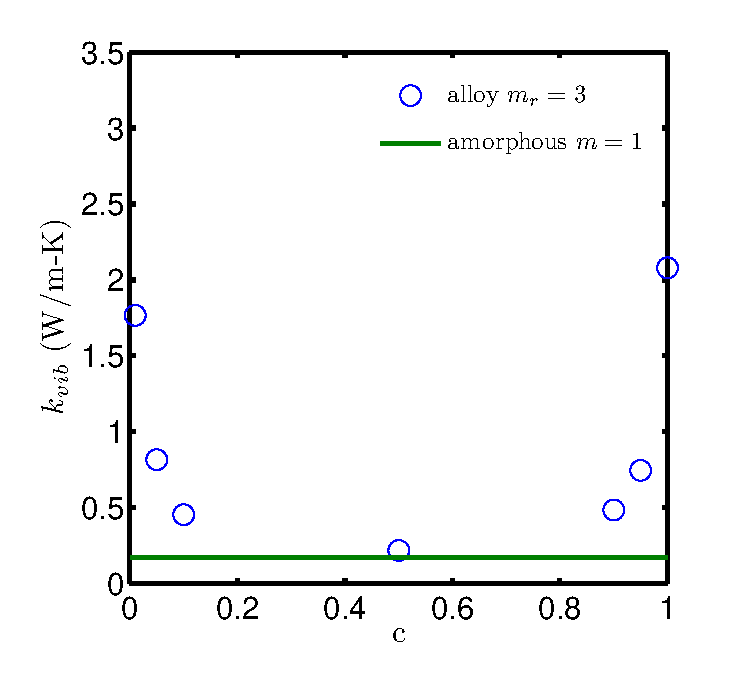
\includegraphics[scale=0.6]
{/home/jason/thesis/proposal/paper/LJ_alloy_GK.eps}
\vspace*{-5mm}
\end{center}
\caption{\label{FIG:gk_alloy} The vibrational conductivity of LJ alloys 
predicted using MD simulations and the Green-Kubo method. The predicted 
thermal conductivities are for a LJ alloy of the form $m^a_{1-c}m^b_{c}$, 
where $m^a =$ 1, $m^b=$ 3, and $m_r = m^a/m^b=$ 3 (in LJ units). As the 
alloy concentration is increased perturbatively, the vibrational 
conductivity drops quickly and saturates to a minimum at $c=0.5$. For 
$c=0.5$ the system is heavily disordered and the vibrational conductivity 
approaches that of an amorphous system.}
\end{figure}
%--------------------------------------------------------------------------

%--------------------------------------------------------------------------
\subsection{\label{S:}From NMD and ALD using VC}
%--------------------------------------------------------------------------

%--------------------------------------------------------------------------
\subsection{\label{S:}NMD and ALD Lifetime Comparison}
%--------------------------------------------------------------------------
Essentially, the normal mode mappings are performed using eigenvectors 
which are plane waves.\cite{}
%--------------------------------------------------------------------------
\section{\label{S:}Discussion}
%--------------------------------------------------------------------------
- compare lifetimes from 2 atom alloy, 4 atom alloy.  Is the reduction in 
thermal conductivity mostly due to the reduction in group 
velocities/introduction of optical modes?
%--------------------------------------------------------------------------
\subsection{\label{S:}Boundary Scattering}
%--------------------------------------------------------------------------
Boundary scattering is responsible for decreasing the long lifetimes 
(mean free paths) of low frequency phonons which carry a significant 
amount of heat, making it particularly effective at decreasing the 
thermal conductivity of systems with length scale of 100s of nm and 
less.\cite{mcgaughey_nanostructure_2012}

First-principles calculations on some thermoelectric
materials show that phonons have a wide MFP distribution,
and hence relatively large nanostructures can reduce their
lattice thermal conductivity.5,18,19 On the other hand, recent
first-principles calculations have shown that the distribution is
much narrower for PbTe,20 and thus, further characterizations
of the distributions and the associated detailed heat conduction
of lead chalcogenides are important for better material design.
%--------------------------------------------------------------------------
\section{\label{S:}Summary}
%--------------------------------------------------------------------------


%--------------------------------------------------------------------------
\appendix
%--------------------------------------------------------------------------
\section{\label{A:}Predicted Phonon Properties: NMD vs ALD}
%--------------------------------------------------------------------------

%--------------------------------------------------------------------------
\subsection{\label{A:}Ioffe-Regel Limit on Phonon Lifetimes}
%--------------------------------------------------------------------------
For defects, the lifetimes can be reduced down to the Ioffe-Regel limit. 
Compare $D = v_s^2 1/\omega$ with  $D = v_s a $
%--------------------------------------------------------------------------
\section{\label{A:}Allen-Feldman Diffuson Theory}
%--------------------------------------------------------------------------
$k_{AF} = \sum_{modes} c(\omega)D_{AF}(\omega)$ 
%--------------------------------------------------------------------------
\subsection{\label{A:}AF Mode Diffusivity}
%--------------------------------------------------------------------------
Shows that for c=0.5 the AF mode diffusivities agree with VC phonon mode 
diffusivities.
%--------------------------------------------------------------------------
\subsection{\label{A:}AF Mode Velocity}
%--------------------------------------------------------------------------
Demonstrates the importance of a mode-dependent group velocity instead of 
using $v_s$ for all modes.
%--------------------------------------------------------------------------
\subsection{\label{A:}AF Thermal Conductivity Predictions}
%--------------------------------------------------------------------------
Results depend on broadening factor, except for heavily disordered systems 
(c=0.5 and amorphous).

\subsection{\label{A-Phonon-Normal-Modes}Vibrations in Ordered and 
Disordered Solids}
%--------------------------------------------------------------------------
In a crystal (periodic) system, the vibrations of atoms are described by a 
basis of eigenfunctions called phonon normal modes, which are determined by 
the properties of the crystal (see Appendix 
\ref{A-Allowed-Wavevectors-Ordered}). The eigenvalues of this basis are the 
phonon mode frequencies (energies).\cite{dove1993,wallace1972} The atomic 
velocities can be represented by the velocity normal mode coordinate, 
defined as 
\cite{dove1993}
\begin{equation}\label{E:udot_HLD}
\begin{split}
\dot{u}_{\alpha}\lbt = &\SUMprime{2}{} \frac{1}{\sqrt{m_bN}} 
\EXP{i\pmb{\kappa}^{'}\cdot\mathbf{r}_0\ab{l}{0}} e^*\kvba 
\dot{q}\kvt{}{}{}.
\end{split}
\end{equation}
Here, $\dot{q}\kvt{}{}{}$ represents the kinetic energy $T \kvt$ of the 
mode with phonon frequency $\omega_0\kv$ by
\cite{dove1993}
\begin{equation}\label{E:udot_HLD}
\begin{split}
T \kvt= \frac{\dot{q}^*\kvt{}{}{}\dot{q}\kvt{}{}{}}{2}.
\end{split}
\end{equation}
The phonon mode kinetic energies $T \kvt$ are used to calculate the phonon 
spectral energy denisty in Appendix \ref{A-Phonon-Life-SED}.

\subsection{\label{A-Allowed-Wavevectors-Ordered}Allowed Wavevectors in 
Ordered Systems}
%--------------------------------------------------------------------------
The phonon spectral energy is defined for the allowed wavevectors of a 
crystal, which can be specified from the crystal structure's Bravais 
lattice and its basis, i.e. unit cell. A $D$-dimensional Bravais lattice 
is a collection of points with
positions
\begin{equation}\label{crys_pos}
\begin{split}
\mathbf{u}_0\ab{l}{0} =& \sum^D_{\alpha} N_{\alpha}\mathbf{a}_{\alpha}
\end{split}
\end{equation}
where $N_{\alpha}$ and the summations if over the lattice vectors, 
$\mathbf{a}_{\alpha}$.\cite{ashcroft1976} The basis (or unit cell) is the 
building block of the crystal and they are arranged on the points defined 
by the Bravais lattice. The equillibrium position of any atom in the crystal 
can be described by
\begin{equation}\label{crys_pos2}
\begin{split}
\mathbf{u}_0\ab{l}{b} = \mathbf{u}_0\ab{l}{0} + \mathbf{u}_0\ab{0}{b}
\end{split}
\end{equation}
where $\mathbf{u}_0\ab{l}{0}$ is the equilibrium position of the 
$l^{\textrm{th}}$ unit cell and $\mathbf{u}_0\ab{0}{b}$ is the equilibrium 
position of the and $b^{\textrm{th}}$ atom in the unit cell relative to 
$\mathbf{u}_0\ab{l}{0}$.
For the LJ systems studied here, the cubic conventional cells are used with 
four atoms per unit cell.\cite{ashcroft1976} For our MD simulations, cubic 
simulation domains with periodic boundary conditions are used with 
$N_1 = N_2 = N_3 = N_0$.\cite{turney2009a,mcgaughey2004a} The allowed 
wavevectors for such crystal structures are
\begin{equation}\label{crys_pos3}
\begin{split}
\pmb{\kappa} = \sum_{\alpha} \mathbf{b}_{\alpha} 
\frac{n_{\alpha}}{N_{\alpha}},
\end{split}
\end{equation}
where $\mathbf{b}_{\alpha}$ are the reciprocal lattice 
vectors\cite{ashcroft1976} and $-N_{\alpha}/2 < n_{\alpha} 
\leq N_{\alpha}/2$, where $n_{\alpha}$ are integers and $N_{\alpha}$ 
are even integers.\cite{turney2009a} The wavevectors are taken to be 
in the first Brioullin zone.\cite{ashcroft1976}

%--------------------------------------------------------------------------
\subsubsection*{Allowed Wavevectors in Disordered Materials}
%--------------------------------------------------------------------------
Strictly speaking, the only allowed wavector in a disordered system is the 
gamma point ($\kappa = [0 0 0]$). As such, the lattice dynamics calculations 
are performed at the gamma point:
%--------------------------------------------------------------------------
\subsection{\label{S:Lifetimes:}Normal Mode Decomposition}
%--------------------------------------------------------------------------
Normal mode decomposition and its limitations.
\cite{turney_predicting_2009-1} 

If $\gamma \kv > \omega \kv$, then the vibrational mode is overdamped.  
Discuss why real-space method is necessary in this case.
%--------------------------------------------------------------------------
\section{\label{A-Finite-Sim}Finite Simulation-Size Scaling for Thermal 
Conductivity}
%--------------------------------------------------------------------------
For the LJ argon system studied in Section \ref{S-Prelim-Vib-Cond-Ordered}, 
a finite simulation-size scaling procedure\cite{turney2009a,He2011a} is 
used to compare the thermal conductivity predictions from $\Phi$ and $\Phi'$ 
to those from the Green-Kubo method. The scaling procedure is demonstrated in 
Fig$.$ \ref{FIG:LJ_COND}. The thermal conductivity is predicted from $\Phi$ 
or $\Phi'$ and MD simulations with $N_0 = 4,6,8,$ and $10$. The bulk 
conductivity, $k_{\infty}$, is then estimated by fitting the data to
\begin{equation}\label{k_size}
\begin{split}
1/k = 1/k_{\infty} + A/N_0,
\end{split}
\end{equation}
where $A$ is a constant. This procedure is necessary because the first 
Brillouin zone is only sampled at a finite number of points for a finite 
simulation size, with no contribution from the volume at its center. To 
predict a bulk thermal conductivity, it is important to sample points near 
the Brillouin zone center, where the modes can have large lifetimes and 
group velocities.\cite{turney2009a,sellan2010b} 

%--------------------------------------------------------------------------
\begin{figure}
\begin{center}
%\includegraphics[angle=0,width=70.0mm]{LJ_NMD_SED_COND_2.eps}
\end{center}
\caption{\label{FIG:LJ_COND} Thermal conductivity predictions for LJ argon calculated using phonon lifetimes predicted by $\Phi$ and $\Phi'$.\cite{Larkin2012} (a) The finite simulation-size scaling extrapolation \cite{turney2009a,He2011a} is used to compare the results to bulk predictions made using the Green-Kubo method. (b) The bulk results for $\Phi$ and Green-Kubo are in good agreement temperatures of $20$ and $40$ K with those of other atomistic simulation methods.\cite{turney2009a}}
\end{figure}
%--------------------------------------------------------------------------


\clearpage
\bibliographystyle{apsrev}
\bibliography{/home/jason/ntpl-ref/ntpl-jason/ntpl-jason-092012}
\end{document}
